\chapter{Christ Speaks to His Churches (2:1--3:13)}
\normalsize

\section{The World of the Early Church}

The years that John wrote Revelation were among the most powerful in the history of the Roman Empire\index{Roman Empire}. Earthly rulers appeared nearly invincible, their authority reaching across vast territories and their power beyond challenge.

It was in this very age that God established the early Church. Believers came to know the true King, Jesus Christ, and bore witness to Him, even at the cost of their lives.

Emperor worship\index{emperor worship} gradually became part of public life. Religious policies, however, were not entirely uniform across the empire. As long as they were not perceived as threats to public order, many peoples were permitted to retain their traditional religious practices. Judaism, with its long history, enjoyed a degree of religious privilege under Roman rule, allowing Jewish communities to worship\index{worship} the God of their ancestors according to their established laws and customs. 

Christianity initially emerged from this Jewish setting, and in some places Christians were regarded as part of the broader Jewish tradition. As Christianity gradually became more distinct from Judaism, however, the protection afforded by that inherited religious status diminished.\footnote{Beale, G. K. (1999).}

Christians worshiped the one true God and confessed Jesus Christ as Lord. They could not, therefore, worship the emperor as a god. This refusal could expose them to social hostility and official pressure. In some regions, they faced the danger of confiscation of property, exile, imprisonment, or even execution.

\begin{figure}[htbp]
    \centering
    \caption{Timeline of Roman Emperors, AD 1--138}
    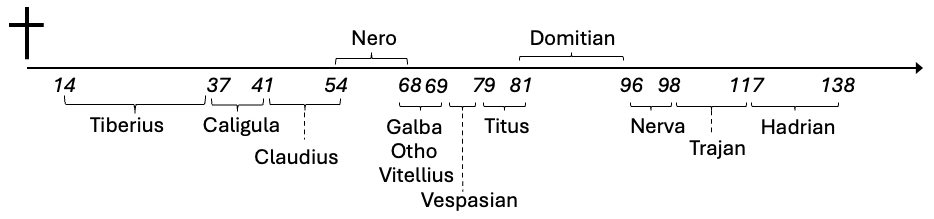
\includegraphics[
    width=1\textwidth,
    trim=0 0 0 0,
    clip]{images/roman_emperors.png}
    \label{fig:roman_emperors}
\end{figure}

I drew a timeline of Roman emperors from AD 1 to 138 in Figure~\ref{fig:roman_emperors}.
Among these emperors, Nero\index{Nero} and Domitian\index{Domitian} are often remembered in historical accounts as tyrants. Both concentrated power in their own hands, suppressed political rivals, and executed opponents, sometimes under charges such as treason. Nero is especially remembered for persecuting Christians after the Great Fire of Rome\index{Rome} in AD 64. Table \ref{table:nero_domitian} highlights the facts.\footnote{As for Domitian, ancient sources describe his suppression of dissent, but scholars continue to debate whether he conducted a large-scale persecution of Christians.}


{
\small
\begin{longtable}{|p{2.5cm}|p{6.5cm}|}
\caption{Nero and Domitian: persecution and rule}
\label{table:nero_domitian} \\
\hline
\textbf{Emperor}\footnote{The portrait of Nero is held by the Glyptothek in Munich; the portrait of Domitian is held by the Louvre in France.}
&
\textbf{Persecution and Rule}
\\
\hline

\centering
Nero

\includegraphics[
    width=\linewidth,
    trim=0 0 0 0,
    keepaspectratio
]{images/nero.jpg}

&
\vspace{-0.3cm}
\begin{itemize}[nosep, leftmargin=10pt]
\item Executed political rivals and members of the Senate.
\item Used legal charges, including treason, to suppress opponents.
\item Ordered the murder of his own mother, Agrippina.
\item Persecuted Christians following the Great Fire of Rome in AD 64.
\item Ruled through fear, violence, and arbitrary power.
\item Those who refused to participate in emperor worship could be accused of atheism or impiety.
\end{itemize}
\\[-0.5cm]
\hline

\centering
Domitian

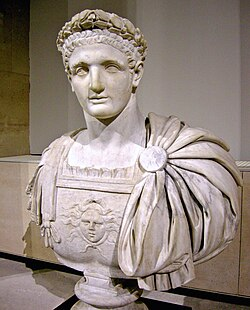
\includegraphics[
    width=\linewidth,
    keepaspectratio
]{images/domitian.jpeg}

&
\vspace{-0.3cm}
\begin{itemize}[nosep, leftmargin=10pt]
\item Executed senators and political opponents.
\item Used legal charges, including treason, to suppress rivals.
\item Confiscated the property of convicted opponents.
\item Was associated with the title ``Lord and God'' (\textit{Dominus et Deus}), which Suetonius says was used in addressing him.\footnote{Suetonius. (1914). \textit{Lives of the Caesars: Volume II} (J. K. Rolfe, Trans.). Harvard University Press.}
\item Those who refused to participate in emperor worship could be accused of atheism or impiety.
\item Ruled through suspicion, informants, and repression.
\end{itemize}
\\
\hline
\end{longtable}
}

Against this backdrop of persecution\index{persecution}, let us turn to the letters Jesus addressed to the seven churches\index{seven churches}. The locations of the seven churches can be seen in Figure~\ref{fig:turkey-seven-churches}.

\normalsize

\subsection{Why These Seven Churches?}\index{seven churches}

A reader's first question may be this: Why these seven churches\index{seven churches}? The New Testament also mentions churches in Rome\index{Rome}, Corinth, Philippi, Colossae, Thessalonica, and many other cities. Why are they not included here?

The seven churches\index{seven churches} in Revelation were not chosen at John's own discretion. Christ commanded him: ``Write on a scroll\index{scroll} what you see and send it to the seven churches'' in Asia.

The number seven appears repeatedly throughout Revelation and often conveys a sense of completeness. These letters, therefore, were not intended only for the seven congregations that first received them. Each letter concludes with the call to hear what the Spirit says to the churches. What Christ says to one congregation is thus also a message to the wider Church.

To help readers enter the world of these early believers, I have designed a series of imagined conversations between brothers in the faith. Through these dialogues, we may almost step into the churches themselves and listen to how their members understood their circumstances before hearing Christ speak to them.

Each of the seven letters contains Christ's commendation, rebuke, command, and promise. For clarity, I have organized His message under four headings: ``Christ's Commendation,'' ``Christ's Rebuke,'' ``Christ's Command,'' and ``Christ's Promise.''

One detail deserves special attention: two churches receive no commendation at all. The word ``None'' is sobering, even painful. If the Lord were to speak directly to our own churches, would we hear His commendation? Or would we, too, be confronted with that heartbreaking word: ``None''?

\section{The Church in Ephesus (2:1--2:7)}\index{Ephesus}

\begin{DialogueBox}
\noindent\faUser\ Brother One: ``Through the years, our brothers have labored for the Lord's name, endured hardship, and refused to turn back when persecution\index{persecution} came. When people taught strange doctrines, we examined their claims. When men called themselves apostles, we did not accept them without testing them. ''

\vspace{0.1cm}

\noindent\faUser\ Brother Two: ``We have indeed done much in the Lord's name. And yet, at times, I remember the days when we first believed. The brothers and sisters loved one another with such fervor. We gathered eagerly to hear the word, to pray, and to break bread together. But I wonder whether the love we once had for the Lord and for one another has quietly grown cold.''
\end{DialogueBox}

\subsection{Geographical Background}

Ephesus\index{Ephesus}, the city in which this church was established, was prosperous and deeply shaped by the worship of idols.

Visitors to the ruins of ancient Ephesus\index{Ephesus} today can still see the remains of its great theater, Harbor Street, Marble Road, marketplaces, library, temples, and fountains. Walking among these surviving stones, we can begin to imagine the city's former splendor as one of the important centers of the Roman Empire\index{Roman Empire}.

The Temple\index{temple} of Artemis was one of the most important symbols of Ephesian identity. Artemis was the Greek name of the goddess whom the Romans called Diana. Worship of Artemis was more than a religious practice; it also sustained related trades and commercial activities. Acts 19:24 tells us that a silversmith named Demetrius made silver shrines of Artemis, bringing considerable business to the craftsmen.

Then Paul and his companions began proclaiming the gospel in Ephesus\index{Ephesus}. Many people abandoned their idols and turned to Christ. As the gospel transformed lives, it also began to affect the social and economic activities built around idol worship.

Demetrius gathered fellow silversmiths and other craftsmen, accusing Paul and his companions of threatening the honor of Artemis and endangering their livelihood. The whole city was thrown into an uproar. A crowd rushed into the theater and, for about two hours, shouted, ``Great is Artemis of the Ephesians!''

Luke, the physician, records the confusion with a touch of understated irony: the assembly was in disorder, some shouting one thing and others another, and most of the people did not even know why they had gathered (Acts 19:28, 32, 34).

Imagine the multitude filling that enormous theater, shouting for two uninterrupted hours. The scene gives us a sense not only of the scale of Ephesus\index{Ephesus} but also of the intensity of its religious devotion and the central place idol worship occupied in civic life.

It was in this prosperous, influential city, so deeply entangled with the worship of idols, that Christ established His Church.


The church in Ephesus\index{Ephesus} was prominent among all the early churches.
Paul's letter to the Ephesians opens with a magnificent declaration of God's predestination: God chose His people in Christ before the creation of the world (Ephesians 1:4). Paul then unfolds the great mystery God has accomplished in Christ.

That \textit{mystery} is the Church: through the gospel, Gentiles are fellow heirs, members of the same body, and sharers together in the promise in Christ Jesus (Ephesians 3:6).\footnote{The church is called a mystery, one not revealed to the Old Testament saints. Also, see Figure \ref{fig:valley}
in Appendix~\thechapter~ ``How Long Is the Great Tribulation?''}
Paul also prays that Christ may dwell in their hearts through faith, that they may be rooted and established in love, and that together with all the saints they may grasp how wide and long and high and deep is the love of Christ (Ephesians 3:17--18).

\subsection{Christ's Commendation}

\begin{ScriptureBox2}{How does Christ introduce Himself in 2:1? Underline everything He knows and commends about the church.}
% Insert the NIV text of Revelation 2:1--3 here.
\item[2:1] Christ is presented as the One who holds the seven stars in His right hand and walks among the seven golden lampstands.

\item[2:2] He knows the church's deeds, hard work, perseverance, intolerance of wickedness, and careful testing of those who claim to be apostles but are not.

\item[2:3] He commends the believers for enduring hardship for His name and not growing weary.
\end{ScriptureBox2}

These were believers whose faith was expressed through action. They labored for the Lord, endured hardship, guarded the truth, and learned to distinguish truth from error.

When Paul took leave of them, the elders of the Ephesian church wept openly. What grieved them most was his declaration that they would never see his face again (Acts 20:38).

Paul had also solemnly warned them to remain alert, because savage wolves would come among them and would not spare the flock (Acts 20:29). The Ephesian believers had truth, diligence, perseverance, and love. They had much for which to be commended.

\subsection{Christ's Rebuke}

\begin{ScriptureBox2}{What does Christ hold against the church?}
% Insert the NIV text of Revelation 2:4 here.
\item[2:4] Christ rebukes the church because it has forsaken the love it had at first.
\end{ScriptureBox2}

Yet some thirty years after the Church's earliest days, Christ spoke through John and declared that the Ephesians had forsaken their first love.

By this time, the congregation may have included believers of the second or even third generation. Sound teaching remained. The church continued to serve, and its members were still known for their perseverance. From a human perspective, it might have appeared to be a model congregation.

Yet something was quietly slipping away: the love that had marked its beginning.

This is what makes the Ephesian church so searching an example for us. A church may stand firmly for truth, labor tirelessly for the Lord, and endure hardship without surrendering. And yet, almost without noticing, it may lose the love that once gave life and warmth to all its work.

\subsection{Christ's Command}

\begin{ScriptureBox2}{Circle the three things Christ commands the church to do in 2:5. What will happen if they do not repent?}
% Insert the NIV text of Revelation 2:5--6 here.
\item[2:5] Christ calls the church to remember how far it has fallen, repent, and do the things it did at first. He warns that, without repentance, He will remove its lampstand from its place.

\item[2:6] He commends the church for hating the practices of the Nicolaitans, which He also hates.
\end{ScriptureBox2}

How can love that has grown cold be restored? The answer is \textbf{repentance\index{repentance}.}

Repentance awakens a heart that has grown indifferent and rekindles a love that has faded. However far we may have wandered, grace\index{grace} can still turn us around and renew us in the Lord.

Repentance is more than sorrow over past failures. It is a renewed turning toward Christ, a return to the life of loving Him and following Him as we did at the beginning.

We need to repent daily. As the Lord Jesus taught His disciples, we must take up our cross daily and follow Him (Luke 9:23).

It is important to notice that Christ's rebuke does not mean the Ephesian church had compromised the truth. On the contrary, the believers continued to hate the practices of the Nicolaitans\index{Nicolaitans}, and Christ commended them for this. We cannot identify with certainty the precise background or teaching of the Nicolaitans.\footnote{MacArthur, J. (2007).} Nevertheless, their practices represented teachings and behaviors that Christ condemned.

\subsection{Christ's Promise}

\begin{ScriptureBox2}{What does Christ promise to the one who is victorious, and where is it found?}
% Insert the NIV text of Revelation 2:7 here.
\item[2:7] The Spirit calls everyone who has ears to hear what He says to the churches. To the one who is victorious, Christ promises the right to eat from the tree of life in God's paradise.
\end{ScriptureBox2}

The tree of life\index{tree of life} immediately brings us back to Genesis 2--3, while the paradise promised here anticipates Revelation 22:1--5.

From Genesis to Revelation, we see the unfolding of one great story: humanity loses Eden\index{Eden}, redemption\index{redemption} is accomplished through Christ, the victorious enter God's paradise, and God's people finally dwell with Him in the new heaven and new earth\index{new heaven and new earth}.

Christ does not merely call His Church to remain faithful on earth. He will ultimately bring His people into glory\index{glory}.

The struggles, repentance\index{repentance}, endurance, and faithfulness of the Church today are not the end of the story. The story reaches its fulfillment in the eternal presence of God. Christ's promise to Ephesus\index{Ephesus} therefore speaks both to the church's present condition and to the glory toward which He is leading His people.

\section{The Church in Smyrna (2:8--2:11)}\index{Smyrna}

\begin{DialogueBox}
\noindent\faUser\ Brother One: ``We in Smyrna\index{Smyrna} are afflicted and poor by the standards of this world. Some have been slandered because of their faith in Christ. Some of our brothers have already given their lives for the Lord's name. And yet, we still gather to worship Him. If we can remain faithful to Christ, what does earthly poverty matter?''

\vspace{0.1cm}

\noindent\faUser\ Brother Two: ``In the eyes of the world, we may possess almost nothing. But there is one thing we must never surrender: our faithfulness to the Lord. The suffering ahead may be greater than anything we have yet endured. But we belong to Christ. We must hold fast to Him to the end.''
\end{DialogueBox}

\subsection{Geographical Background}

Smyrna\index{Smyrna} is modern-day Izmir, Turkey's third-largest city and an important port on the Aegean coast. Traces of its long history remain visible today, including the ancient agora, Roman-era colonnades, public buildings, and other urban structures.

In Roman times, Smyrna\index{Smyrna} was known for its loyalty to Rome\index{Rome}. As early as approximately 195 BC, the city established a temple\index{temple} dedicated to Roma, the personification of Rome, as a public expression of its allegiance. Later, in AD 26, Smyrna competed with other cities of Asia and won permission to build a temple honoring Emperor Tiberius, Livia, and the Roman Senate.

Against this background, Christians who refused to participate in emperor worship\index{emperor worship} could be viewed as refusing to demonstrate loyalty to Rome\index{Rome}. For the believers in Smyrna\index{Smyrna}, confessing with their hearts and mouths that Jesus is Lord was therefore no trivial matter. It could become a question of livelihood, freedom, and even life itself.

This setting helps us understand how precious Christ's commendation of the church in Smyrna\index{Smyrna} truly was.

\subsection{Christ's Commendation}

\begin{ScriptureBox2}{How does Christ describe Himself in 2:8? What does He know about the church, and how does He see its poverty?}
% Insert the NIV text of Revelation 2:8--9 here.
\item[2:8] Christ identifies Himself as the First and the Last, who died and came to life again.

\item[2:9] He knows the church's affliction and poverty, yet declares it spiritually rich. He also knows the slander spoken by those who claim to be Jews but are described as a synagogue of Satan.
\end{ScriptureBox2}

The church in Smyrna\index{Smyrna} became known for its steadfast faithfulness, even unto death.

Around AD 155--160, Polycarp served as bishop of Smyrna\index{Smyrna}. According to early Christian tradition, he had been acquainted with the apostle John. Polycarp was arrested and brought before the authorities. When ordered to deny Christ, he reportedly answered, ``For eighty-six years I have served him, and he has done me no wrong. How can I blaspheme my King who saved me?''\footnote{\textit{Martyrdom of Polycarp}. (1885). (A. Roberts \& J. Donaldson, Trans.). Christian Literature Publishing. (Original work published ca. 155).}

His martyrdom\index{martyrs} became one of the best-known testimonies of faith in early Christianity.

Smyrna\index{Smyrna} was a city celebrated for its loyalty to Rome\index{Rome}. Yet within that city, Christ had established a people whose ultimate allegiance belonged to Him alone.

\subsection{Christ's Rebuke}

None.

\subsection{Christ's Command}

\begin{ScriptureBox2}{What are the believers told not to fear, and how long will their testing last? What are they commanded to do?}
% Insert the NIV text of Revelation 2:10a here.
\item[2:10a] Christ tells the believers not to fear the suffering ahead. Some will be imprisoned and tested, and they will face tribulation for a limited period. He commands them to remain faithful, even to the point of death.
\end{ScriptureBox2}

The reference to ten days suggests a period that is limited rather than endless. The suffering may be severe, but it does not continue without limit, nor does it escape the sovereign rule of God.

\subsection{Christ's Promise}

\begin{ScriptureBox2}{What two things does Christ promise to the one who is victorious?}
% Insert the NIV text of Revelation 2:10b--11 here.
\item[2:10b] Christ promises the crown of life.

\item[2:11] The one who is victorious will not be hurt by the second death.
\end{ScriptureBox2}

The ``second death\index{second death}'' refers to the final judgment\index{judgment} and eternal punishment (Revelation 20:14).

Victory does not mean that believers earn salvation through their own courage or perseverance. Rather, it describes the faithfulness of those who belong to Christ and continue to hold fast to Him through suffering, sustained by His grace.

For the church in Smyrna\index{Smyrna}, this promise was especially precious. Some believers might be killed because they refused to deny Christ. Yet physical death could not undo the eternal life He had given them.

The One who died and came to life again had already conquered\index{overcomers} death. Those who belong to Him will not suffer the second death\index{second death}. They may lose their earthly lives, but they will never lose the eternal life Christ has promised.

\section{The Church in Pergamum (2:12--2:17)}\index{Pergamum}

\begin{DialogueBox}
\noindent\faUser\ Brother One: ``What a prosperous city Pergamum\index{Pergamum} is, with its many temples and its constant stream of sacrifices. Yet the people here invite us to their banquets, where sacrifices are offered to idols. We cannot always refuse such invitations without consequence. Perhaps we can hold fast to our faith while making a few small concessions elsewhere.''

\vspace{0.1cm}

\noindent\faUser\ Brother Two: ``I have thought the same way. Some brothers say that, as long as we continue to trust Christ in our hearts, it should be harmless to attend these feasts from time to time and eat food sacrificed to idols. But lately my conscience has grown troubled. We were called to turn from idols and come to the Lord. If we keep yielding, little by little, are we preserving our lives—or slowly abandoning the way of Christ?''
\end{DialogueBox}

\subsection{Geographical Background}

Pergamum\index{Pergamum}, known today as Bergama, lies in western Turkey, in Izmir Province. Its ancient ruins are now recognized as a UNESCO World Heritage Site.

Visitors can explore the city's acropolis, perched high on a hill, where the remains of an ancient theater, the Temple\index{temple} of Athena, a library, the altar\index{altar} of Zeus, and a temple associated with the Roman emperor Trajan can be seen. The nearby Asclepion was a celebrated center of ancient medicine and healing, and remains one of the region's most important archaeological sites.

Pergamum\index{Pergamum} was also famous for its library and for parchment, the writing material whose name is derived from the city's own name. It was an important center of learning in the ancient world. Under Roman rule, it became a major city in the province of Asia and an important center of imperial cult\index{emperor worship} activity.

\begin{figure}[htbp]
    \centering
    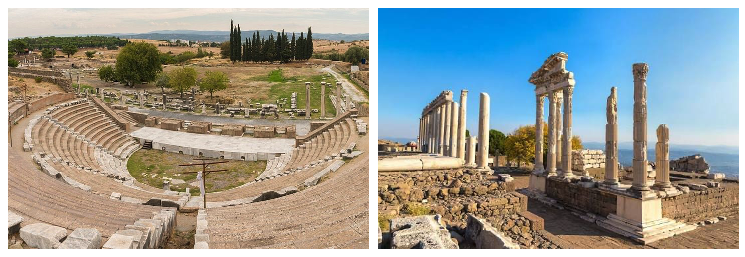
\includegraphics[
    width=1\textwidth,
    trim=0 0 0 0,
    clip]{images/pergamum3.png}
    \caption{The ancient theater and remains associated with the Altar of Zeus at Pergamum}
    \label{fig:pergamum3}
\end{figure}

\subsection{Christ's Commendation}

\begin{ScriptureBox2}{How does Christ introduce Himself in 2:12? Where do these believers live, and what did they do even when Antipas was killed?}
% Insert the NIV text of Revelation 2:12--13 here.
\item[2:12] Christ introduces Himself as the One who has the sharp, double-edged sword.

\item[2:13] He knows where the believers live, in a place described as Satan's throne. Even when His faithful witness Antipas was killed there, the church held firmly to Christ's name and did not renounce its faith.
\end{ScriptureBox2}

Pergamum\index{Pergamum} was not merely a center of culture and learning. It was also a city steeped in religious activity and imperial worship. This background helps explain the force of Christ's description of it as the place ``where Satan\index{Satan} has his throne\index{throne of God}'' (Revelation 2:13).

\subsection{Christ's Rebuke}

\begin{ScriptureBox2}{Whose teachings do some in the church hold to? Underline what Balaam led Israel into.}
% Insert the NIV text of Revelation 2:14--15 here.
\item[2:14] Christ rebukes the church because some hold to the teaching of Balaam, who taught Balak to entice Israel into eating food sacrificed to idols and committing sexual immorality.

\item[2:15] Some also hold to the teaching of the Nicolaitans.
\end{ScriptureBox2}

Numbers 25 describes how Israel\index{Israel} was led into sexual immorality with Moabite women and drawn into idol worship. The episode became a warning about the danger of abandoning faithfulness to God under the influence of surrounding peoples.

Israel had once faced the temptation to compromise in a pagan environment. The church in Pergamum\index{Pergamum} was now confronting a similar danger.

The problem was not new. Israel had faced it in the wilderness, and now the Church was in danger of repeating the same story.

In our own day, this may take the form of teaching and discipleship that encourage compromise: the suggestion that we can retain the language of faith while gradually accommodating practices that draw us away from Christ. Such teaching calls for careful discernment.

\subsection{Christ's Command}

\begin{ScriptureBox2}{What does Christ command, and what will He do if the church does not obey?}
% Insert the NIV text of Revelation 2:16 here.
\item[2:16] Christ commands the church to repent. Otherwise, He will come and fight against those who persist in error with the sword of His mouth.
\end{ScriptureBox2}

As discussed in Table~\ref{tab:christ-revelation-1-3} in Chapter 1, the sword from Christ's mouth represents His authority to judge falsehood and error by His word. Here, He calls the church to turn away from corrupt teaching and conduct and to renew its allegiance to Him.

\subsection{Christ's Promise}

\begin{ScriptureBox2}{What two gifts does Christ promise to the one who is victorious, and what is written on the stone?}
% Insert the NIV text of Revelation 2:17 here.
\item[2:17] The one who is victorious will receive hidden manna and a white stone bearing a new name, known only to the one who receives it.
\end{ScriptureBox2}

Manna first calls to mind the food God provided for Israel\index{Israel} in the wilderness (Exodus 16:15). In a city crowded with pagan worship and hostile pressures, Christ promises His victorious people a different kind of nourishment. Their true sustenance will not come from compromising with idols, but from Christ Himself.

The white stone is often understood in light of Roman customs. In some ancient settings, a white token could signify a favorable verdict, recognition, or admission to a special gathering. One proposed interpretation connects it with athletic victory: a victor might receive a token bearing his name that granted entry to a celebratory banquet.\footnote{MacArthur, J. (2007).} Although the precise background remains uncertain, the image clearly conveys welcome and honor bestowed upon the recipient.

In Scripture, a new name often signifies a renewed identity and a new relationship with God. Christ's promise therefore points to the deeper nourishment and lasting identity He gives to those who remain faithful to Him.

\section{The Church in Thyatira (2:18--2:29)}\index{Thyatira}

\begin{DialogueBox}
\noindent\faUser\ Brother One: ``Our brothers and sisters in Thyatira\index{Thyatira} labor diligently. We love one another, and our faith and perseverance have grown. The charitable work we have recently begun is flourishing, and we are finding new ways to serve our neighbors through the city's trades and associations. If we remain loyal to the Lord while living peaceably with those around us, surely we can bear a good witness here.''

\vspace{0.1cm}

\noindent\faUser\ Brother Two: ``I hope that is so. Yet some things trouble my heart. At the gatherings organized by the trade associations, sacrifices to idols are often offered. And our own church has even welcomed a woman who calls herself a prophet, Jezebel\index{Jezebel}, to teach us. She says that believers may participate in eating food sacrificed to idols.''
\end{DialogueBox}

\subsection{Geographical Background}

Thyatira\index{Thyatira}, also spelled Thyateira, is located in the area of modern Akhisar in western Turkey. It was not especially renowned for monumental political power or for being a major religious center. Instead, it was known for commerce and skilled craftsmanship.

Archaeological evidence points to numerous trade associations, or guilds, in Thyatira\index{Thyatira}, including those of wool workers, dyers, linen workers, leatherworkers, and metalworkers. Lydia, mentioned in Acts 16:14, was a seller of purple cloth from Thyatira. She met Paul in Philippi and later became a Christian.

These guilds were more than professional associations. They also served as social networks and could be closely connected with sacrifices to local deities and religious banquets. Participation in guild life could therefore place Christians under pressure to join practices incompatible with their faith.

Thyatira\index{Thyatira} was known for its metalworking traditions. The description of Christ's feet as being like glowing bronze may have resonated with a community familiar with fine metalwork. The precise alloy intended by the original term is uncertain, but the image conveys the brilliance, strength, and purity of refined metal.\footnote{Osborne, G. R. (2002).}

\subsection{Christ's Commendation}

\begin{ScriptureBox2}{Circle how Christ describes His eyes and feet. Underline the five things He commends, and notice how the church's recent works compare with its first.}
% Insert the NIV text of Revelation 2:18--19 here.
\item[2:18] Christ is introduced as the Son of God, whose eyes are like blazing fire and whose feet are like burnished bronze.

\item[2:19] He commends the church's deeds, love, faith, service, and perseverance, noting that its more recent works are greater than those it did at first.
\end{ScriptureBox2}

\subsection{Christ's Rebuke}

\begin{ScriptureBox2}{What does Christ hold against the church? What has He given Jezebel, and what does He say all the churches will know?}
% Insert the NIV text of Revelation 2:20--23 here.
\item[2:20] Christ rebukes the church for tolerating the woman called Jezebel, who teaches and misleads His servants into sexual immorality and eating food sacrificed to idols.

\item[2:21] He has given her time to repent, but she is unwilling to turn from her immorality.

\item[2:22] He warns of judgment upon her and those who persist in following her.

\item[2:23] He will strike her followers, so that all the churches will know that He searches hearts and minds and repays each person according to their deeds.
\end{ScriptureBox2}

Jezebel\index{Jezebel} was the foreign wife of Ahab, king of the northern kingdom of Israel\index{Israel}. She promoted the worship of Baal, persecuted\index{persecution} the prophets of the Lord, and became a lasting biblical symbol of idolatry and wickedness (1 Kings 17--21).

By calling a contemporary figure in the church ``Jezebel\index{Jezebel},'' John deliberately invokes this Old Testament history to help his readers recognize the nature of the present danger.

The references to sexual immorality and eating food sacrificed to idols include actual participation in pagan worship and its associated social banquets. In the Old Testament, sexual immorality also frequently serves as a metaphor for Israel's unfaithfulness to the Lord through idolatry.

The central issue, therefore, is whether the Church remains faithful to Christ or compromises its allegiance in order to accommodate the surrounding culture, religion, and centers of power.

\subsection{Christ's Command}

\begin{ScriptureBox2}{To whom is Christ speaking in 2:24? What must they do until He comes?}
% Insert the NIV text of Revelation 2:24--25 here.
\item[2:24] Christ addresses those who have not accepted this teaching or learned what its followers call the deep secrets of Satan. He places no additional burden upon them.

\item[2:25] They must hold fast to what they have until He comes.
\end{ScriptureBox2}

The expression ``the deep secrets of Satan\index{Satan}'' has been interpreted in at least two ways.\footnote{Osborne, G. R. (2002); Beale, G. K. (1999).}

\begin{enumerate}
\item \textbf{An ironic expression.} Christ may be speaking sarcastically about the claims of Jezebel\index{Jezebel} and her followers. They may have boasted of their knowledge of the deep things of God, echoing language such as that found in 1 Corinthians 2:10, while in reality leading believers into spiritual danger.

\item \textbf{A more literal interpretation.} Jezebel\index{Jezebel} may have been teaching principles resembling early forms of Gnostic thought.\footnote{Gnostic thought, in its various forms, often distinguished between the material world and the spiritual realm and emphasized hidden knowledge (\textit{gnosis}) as a means of attaining spiritual insight or salvation. The early Christian writings, including the letters of John, oppose teachings that distort the truth about Christ and the nature of salvation. See \textit{Caught by Grace}, Chapter 7, ``On Gnosticism.''} Under this interpretation, believers may have been encouraged to experience the supposed ``depths'' of Satan\index{Satan}, perhaps through participation in pagan practices, in the belief that such experiences would enable them to overcome\index{overcomers} evil.
\end{enumerate}

The first interpretation appears more likely, particularly because of its possible connection with Revelation 2:9, where those opposing the church are described as a ``synagogue of Satan\index{synagogue of Satan}.'' Nevertheless, both interpretations raise questions about claims to possess special spiritual knowledge.

In simple terms, Gnostic thought refers to a range of ideas that emphasized special or hidden knowledge as a means of discovering divine truth and escaping the limitations of the material world. Under the first interpretation, the expression ``deep things of God'' may be a mocking reference to the esoteric knowledge sought by early Gnostic teachers. Under the second, it may involve people who believed that possessing special knowledge allowed them to engage in sinful behavior without spiritual consequences. Such an attitude resembles the kind of moral presumption opposed in 1 John 1:8--10 and 3:9.

Whatever the precise historical background, Christ's command is unmistakable: the believers must hold fast to what they have received and refuse to compromise their faith.

\subsection{Christ's Promise}

\begin{ScriptureBox2}{What does Christ promise to the one who is victorious? Circle the image of authority in 2:27 and the gift in 2:28.}
% Insert the NIV text of Revelation 2:26--29 here.
\item[2:26] Christ promises authority over the nations to those who are victorious and continue to do His will to the end.

\item[2:27] They will share in His authority, described through the imagery of an iron scepter and shattered pottery.

\item[2:28] He promises to give them the morning star.

\item[2:29] The Spirit calls everyone who has ears to hear what He says to the churches.
\end{ScriptureBox2}

In the context of this letter, victory means remaining faithful to Christ's commands in the face of Jezebel\index{Jezebel}'s teaching, idolatry, and the temptation to compromise.

The image of the iron scepter comes from Psalm 2:8--9, where the Lord grants the nations to His anointed King and speaks of ruling them with an iron scepter. This does not mean that believers become another Christ. Rather, the authority Christ receives from the Father is shared with those who belong to Him. The victorious will reign with Christ.

The Greek verb translated ``rule'' can also carry the sense of shepherding or tending. The image therefore need not suggest nothing more than destructive force; it can also convey the authority of a king who governs under God's sovereign purpose.

The morning star\index{morning star} becomes especially significant later in Revelation, when Christ identifies Himself as ``the bright Morning Star'' (Revelation 22:16). The promise to give the morning star thus points ultimately to Christ Himself. The greatest reward is not merely authority or honor. It is Christ Himself, given to His victorious people.

The church in Thyatira\index{Thyatira} teaches us why the Church must reject the teaching represented by Jezebel\index{Jezebel}. The Lamb\index{Lamb, the} has purchased His people with His own blood and will lead them into glory. Because the Lamb alone is worthy of worship, the Church must not divide its allegiance with idols. It must remain faithful to Christ until He brings His people into His glorious presence.

\section{The Church in Sardis (3:1--3:6)}\index{Sardis}

\begin{DialogueBox}
\noindent\faUser\ Brother One: ``Our church in Sardis\index{Sardis} has a good reputation. Many gather whenever we meet, and people throughout the city know that we belong to Christ. When I see such enthusiasm, I cannot help thinking that we must have accomplished much for the Lord, and that He must surely be with us.''

\vspace{0.1cm}

\noindent\faUser\ Brother Two: ``From the outside, it certainly appears so. Yet a question keeps troubling me: is our inner life as healthy as our outward appearance? Have our prayers before the Lord, our mutual encouragement, and our repentance\index{repentance} from sin grown weak? People say that we are alive. But what do we look like in the eyes of the Lord?''
\end{DialogueBox}

\subsection{Geographical Background}

Sardis\index{Sardis} lay approximately thirty to forty miles southeast of Thyatira\index{Thyatira}. Established around 1200 BC, it was one of the ancient world's oldest cities and later became the wealthy and powerful capital of the Lydian kingdom.

Through commerce and trade, Sardis\index{Sardis} accumulated great wealth. It is also associated with some of the earliest coinage in gold and silver.

Sardis\index{Sardis} had once been a formidable military stronghold and was difficult to conquer\index{overcomers}. One of its most notable early rulers was Gyges, who reigned in the seventh century BC and helped establish the city's wealth and influence. His successor, Croesus, became so renowned for his riches and power that he believed he could challenge Cyrus, king of Persia.

In the centuries that followed, however, Sardis\index{Sardis} suffered repeated military reversals, including defeats that exposed weaknesses in its defenses. It gradually lost the political and military prominence it had once enjoyed. Although the city retained a measure of wealth and commercial activity, its former glory as the capital of a powerful kingdom had faded.

By the first century AD, Sardis\index{Sardis} had become, in many respects, a city living in the shadow of its past. It still possessed the wealth, culture, and reputation inherited from its former greatness, but it was no longer the mighty political and military center it had once been.

Sardis\index{Sardis} also had a substantial Jewish community, with a history that may reach back to the fifth or fourth century BC. This community played a meaningful role in the city's life and reflected the long-standing interaction of different cultural and religious groups there.\footnote{Osborne, G. R. (2002).}

\subsection{Christ's Commendation}

None.

\subsection{Christ's Rebuke}

\begin{ScriptureBox2}{What does Christ hold? What reputation does the church have, and what is its true condition?}
% Insert the NIV text of Revelation 3:1 here.
\item[3:1] Christ, who holds the seven spirits of God and the seven stars, declares that although the church has a reputation for being alive, it is dead.
\end{ScriptureBox2}

The phrase ``you have a reputation of being alive'' points to the church's public standing. In the eyes of others, Sardis\index{Sardis} appeared to be a thriving congregation. Christ, however, exposes its inward condition: its spiritual life has withered.

There is a striking contrast with the city's own history. Sardis\index{Sardis} had once enjoyed a glorious reputation, only to decline gradually while retaining the outward signs of former greatness. This parallel is illuminating, though we should not assume that John called the church dead simply because of the city's history. His judgment rests on Christ's knowledge of the church itself.

\subsection{Christ's Command}

\begin{ScriptureBox2}{Circle every command Christ gives in 3:2--3. What will happen if the church does not wake up?}
% Insert the NIV text of Revelation 3:2--3 here.
\item[3:2] Christ commands the church to wake up and strengthen what remains and is about to die, for its deeds have not been found complete before God.

\item[3:3] He calls them to remember what they received and heard, keep it, and repent. If they do not wake up, He will come like a thief, at an hour they do not expect.
\end{ScriptureBox2}

The church in Sardis\index{Sardis} needed to wake up, strengthen what remained, remember, obey, and repent\index{repentance}.

Outwardly, the congregation still existed. Inwardly, however, its spiritual life was fading. Yet something remained. Christ's command was therefore not simply a declaration of condemnation; it was a call to preserve what was left and restore it to strength.

This was a summons to turn back from the brink of spiritual death.

\subsection{Christ's Promise}

\begin{ScriptureBox2}{Who in Sardis has not soiled their clothes? Underline the three promises in 3:5.}
% Insert the NIV text of Revelation 3:4--6 here.
\item[3:4] A few in Sardis have not soiled their clothes. They will walk with Christ, dressed in white, for they are worthy.

\item[3:5] Those who are victorious will be dressed in white. Christ will never blot out their names from the book of life but will acknowledge them before His Father and His angels.

\item[3:6] The Spirit calls everyone who has ears to hear what He says to the churches.
\end{ScriptureBox2}

\section{The Church in Philadelphia (3:7--3:13)}\index{Philadelphia}

\begin{DialogueBox}
\noindent\faUser\ Brother One: ``We in Philadelphia\index{Philadelphia} are a small church, and our strength is slight. Compared with other congregations, we may seem insignificant. Yet we must hold fast to the Lord's word and never deny His name. Our trials are many, and there is little we can accomplish by our own strength. But if the Lord grants us even a little strength, we must use it faithfully and remain steadfast in His way.''

\vspace{0.1cm}

\noindent\faUser\ Brother Two: ``Yes. We have nothing of our own in which to boast. We seek no praise from people; we desire only to be faithful before the Lord. If He opens a door before us, then we will do all we can through the strength He provides.''
\end{DialogueBox}

\subsection{Geographical Background}

Philadelphia\index{Philadelphia}, known today as Alaşehir in Turkey, lay about thirty miles southeast of Sardis\index{Sardis}. Situated along an important trade route, it was sometimes described as a gateway to the East. Of the seven cities, it was among the latest to be established, probably after 189 BC.

The city's founding is associated with Attalus II Philadelphus, brother of Eumenes II, king of Pergamum\index{Pergamum}. Attalus was known for his deep affection and loyalty toward his brother. His epithet, ``Philadelphus,'' means ``brother-loving,'' and the city came to bear a name associated with brotherly love.

Like Sardis\index{Sardis}, Philadelphia\index{Philadelphia} lay in a seismically active region and was frequently shaken by earthquakes\index{earthquake}. Volcanic activity had also enriched the surrounding soil, making it particularly suitable for vineyards. Viticulture therefore became an important part of the local economy.

Frequent earthquakes nevertheless made life difficult. The great earthquake of AD 17, which devastated Sardis\index{Sardis}, also caused extensive destruction in Philadelphia\index{Philadelphia}. Walls developed cracks, buildings were unsafe, and the possibility of another earthquake shaped everyday life and long-term planning.

Because of the destruction caused by the earthquake of AD 17, the Roman emperor exempted Philadelphia\index{Philadelphia} from tribute for five years, allowing the city to recover economically and rebuild.

Another event, during Domitian\index{Domitian}'s reign, may have dealt a serious blow to Philadelphia\index{Philadelphia} around AD 92. Ancient evidence and later interpretations associate this period with pressure to reduce vineyards and expand grain production, possibly to supply the Roman army or in response to food shortages. The exact details and scope of such an order remain uncertain. Nevertheless, restrictions on vineyards would have been economically damaging: grain was less profitable than wine, and the local volcanic soil was not especially suited to grain cultivation. Because vineyards took years to mature, such restrictions would have threatened the livelihoods of local growers and caused widespread resentment in the province of Asia.\footnote{Osborne, G. R. (2002).}

\subsection{Christ's Commendation}

\begin{ScriptureBox2}{What does Christ hold, and what can He open and shut? Underline what He says about the church's strength and faithfulness.}
% Insert the NIV text of Revelation 3:7--9 here.
\item[3:7] Christ is described as holy and true, the One who holds the key of David. What He opens no one can shut, and what He shuts no one can open.

\item[3:8] He knows the church's deeds and its little strength. The believers have kept His word and have not denied His name. He has placed before them an open door that no one can shut.

\item[3:9] Christ promises to make those who oppose the church recognize that He has loved His people.
\end{ScriptureBox2}

The phrase ``who holds the key of David'' directly echoes Isaiah 22:22, where the key of the house of David is placed upon the shoulder of the appointed steward: what he opens no one can shut, and what he shuts no one can open.

The emphasis is on the authority of the One who holds the key. It is Christ who determines which doors open and which remain shut. The future of the church does not rest ultimately in the hands of earthly powers.

The church's ``little strength'' does not mean that it possesses little spiritual value. Rather, its members lack the outward power, political influence, and economic resources that the world admires. Yet they have kept Christ's word and have not denied His name. Their faithfulness rests not on worldly strength but on the Lord who sustains them.

The expression ``those who claim to be Jews'' refers to people who opposed the church and whose claims to religious identity are challenged by Christ. The passage describes their conduct as false and places them under the judgment of the One who knows the truth.

\subsection{Christ's Rebuke}

None.

\subsection{Christ's Command}

\begin{ScriptureBox2}{Why does Christ promise to keep the church in the time of trial? What does He announce, and what must they hold fast?}
% Insert the NIV text of Revelation 3:10--11 here.
\item[3:10] Because the church has kept Christ's command to endure patiently, He promises to keep them in the time of trial that will come upon the world.

\item[3:11] Christ declares that He is coming soon and commands them to hold fast to what they have, so that no one will take their crown.
\end{ScriptureBox2}

The call to hold fast is grounded in Christ's promise: ``I am coming soon.'' What a profound source of hope. Their endurance is not an exercise in holding on to an uncertain future; it is faithfulness in the light of the coming King.

The promise to keep the church from the time of trial has played an important role in arguments for a pretribulation\index{Rapture!pretribulation view} rapture\index{Rapture}, the view that Christ gathers the Church to Himself before the great tribulation\index{Great Tribulation}.\footnote{MacArthur, J. (2007); Osborne, G. R. (2002).} For a discussion of this and other interpretations, see the appendix, ``When Will the Rapture Take Place?''

\subsection{Christ's Promise}

\begin{ScriptureBox2}{What will the one who is victorious become? Circle the three names Christ will write on that person.}
% Insert the NIV text of Revelation 3:12--13 here.
\item[3:12] The one who is victorious will become a pillar in God's temple and will never leave it. Christ will write upon that person the name of His God, the name of God's city, the New Jerusalem coming down out of heaven, and Christ's own new name.

\item[3:13] The Spirit calls everyone who has ears to hear what He says to the churches.
\end{ScriptureBox2}

Have you ever lived in an earthquake\index{earthquake} zone? Taiwan, for example, lies along an active seismic belt. When an earthquake strikes, even a modern high-rise built with reinforced concrete can seem frighteningly vulnerable. We may imagine the supporting columns cracking and the entire structure collapsing.

Philadelphia\index{Philadelphia} was also located in an earthquake-prone region. Its residents knew what it meant to live with instability, and the church itself had little outward strength. The promise that the victorious would become a pillar in God's temple\index{temple} must therefore have offered them profound comfort.

Christ promises something that no earthquake can destroy: a permanent place in God's presence. Their hope reaches beyond the fragile city in which they live toward the New Jerusalem\index{New Jerusalem} revealed in Revelation 22.

The contrast may be summarized in Table \ref{table:philadelphia_cities}.

{
\renewcommand{\arraystretch}{1}
\begin{longtable}{>{\raggedright\arraybackslash}p{4.5cm}|>{\raggedright\arraybackslash}p{4.5cm}}
\caption{Philadelphia on earth and the city above}
\label{table:philadelphia_cities} \\
\hline
\textbf{Philadelphia on Earth} &
\textbf{The City Above}
\\
\hline
An earthly city &
The New Jerusalem
\\
A city frequently shaken by earthquakes &
God's city, secure forever
\\
Residents may be forced to leave &
The victorious will never leave God's temple
\\
Earthly identity and status may change &
God's name will be written upon His people
\\
Honor derived from belonging to a Roman city &
The glory of belonging to God's eternal city
\\
\hline
\end{longtable}
}

\section{The Church in Laodicea (3:14--3:22)}\index{Laodicea}

\begin{DialogueBox}
\noindent\faUser\ Brother One: ``We in Laodicea\index{Laodicea} have much to be thankful for. Trade flourishes, and many households are prosperous. Through our own labor, we have acquired property and possessions. We lack neither food nor clothing, and life is secure. Even our gatherings for worship lack nothing. We have little persecution\index{persecution} to endure. Surely it is good to live in peace and enjoy the blessings we have received.''

\vspace{0.1cm}

\noindent\faUser\ Brother Two: ``It is true that we lack nothing. But perhaps that is precisely the danger. We do not struggle to survive, nor are we required to pay much for our faith. Have we become too accustomed to a comfortable life?''
\end{DialogueBox}

\subsection{Geographical Background}

Laodicea\index{Laodicea} lay in Phrygia, in western Asia Minor, within the Lycus River valley. Its strategic position made it an important commercial center linking routes between east and west.

Colossae lay approximately ten miles to the east, while Hierapolis was about six miles to the north. Laodicea\index{Laodicea} prospered through trade and finance. It was particularly famous for its black wool, which was soft and dark, like a raven's feathers. The local textile industry became highly successful, giving Laodicea a reputation beyond the surrounding region.

The city was also known for medicine. A renowned medical school was associated with a sanctuary of Men Karou, a Phrygian moon god.\footnote{Men was a Phrygian moon god, and Karoura was the place between Laodicea and Hierapolis where his temple stood.}
Physicians influenced by the medical tradition of Herophilus believed that complex illnesses could be treated with compound remedies. A medicinal preparation for the eyes, known as Phrygian powder, was also associated with the region, adding to Laodicea\index{Laodicea}'s reputation and wealth.

Against this background, Christ's command in Revelation 3:18 to buy eye salve so that the believers might see would have been especially vivid. Readers today may not share the same local associations, but the image is still immediately understandable: a person may possess the means to treat the eyes and yet remain blind to the truth.

Laodicea\index{Laodicea} also lay in an earthquake\index{earthquake}-prone region. Around AD 60, a major earthquake severely damaged the city. Unlike some other cities that depended on imperial assistance, Laodicea rebuilt itself through its own financial resources. This recovery demonstrated the remarkable wealth of its inhabitants.

The surrounding geography offers another striking detail. Hierapolis, to the north, was famous for its hot springs, while nearby Colossae had access to cold, refreshing water. Laodicea\index{Laodicea}, by contrast, relied on aqueducts to bring water from a distance. By the time the water reached the city, it could be lukewarm\index{lukewarm} and mineral-laden, unpleasant to drink.

This local experience gives vivid force to Christ's words: He knows their deeds; they are neither cold nor hot. Because they are lukewarm\index{lukewarm}, He will spit them out of His mouth (Revelation 3:15--16).\footnote{Osborne, G. R. (2002).}

\subsection{Christ's Commendation}

None.

\subsection{Christ's Rebuke}

\begin{ScriptureBox2}{How does Christ describe Himself in 3:14? Underline what the church thinks of itself, then circle Christ's diagnosis and the three things He counsels it to receive.}
% Insert the NIV text of Revelation 3:14--18 here.
\item[3:14] Christ identifies Himself as the Amen, the faithful and true witness, the ruler of God's creation.

\item[3:15--16] He rebukes the church for being neither cold nor hot. Because it is lukewarm, He will spit it out of His mouth.

\item[3:17] The church considers itself wealthy and self-sufficient, not realizing that it is spiritually wretched, pitiful, poor, blind, and naked.

\item[3:18] Christ counsels the church to receive from Him true riches, white clothes to cover its shame, and eye salve so that it may see.
\end{ScriptureBox2}

The problem in Laodicea\index{Laodicea} was that earthly prosperity had been mistaken for spiritual prosperity. Because the believers believed they lacked nothing, they could no longer recognize their need for Christ.

Christ calls them to turn to Him for what they cannot provide for themselves: true riches, a covering for their shame, and sight to recognize their actual condition.

The contrast can be summarized in Table \ref{table:laodicea_diagnosis}.
{
\renewcommand{\arraystretch}{1}
\small
\begin{longtable}{|L{3cm}|L{1.8cm}|L{2.4cm}|L{1.6cm}|}
\caption{Laodicea's self-assessment and Christ's diagnosis}
\label{table:laodicea_diagnosis} \\
\hline
\textbf{Laodicea's Self-Assessment} &
\textbf{Christ's Diagnosis} &
\textbf{Christ's Provision} &
\textbf{Purpose}
\\
\hline
Wealthy &
Poor &
Gold refined by fire &
True riches
\\
\hline
Clothed in fine garments and wool &
Naked &
White garments &
Covering
\\
\hline
Medical knowledge and eye salve &
Blind &
Eye salve &
Sight
\\
\hline
\end{longtable}
}

\subsection{Christ's Command}

\begin{ScriptureBox2}{Whom does Christ rebuke and discipline? What does He call the church to do?}
% Insert the NIV text of Revelation 3:19 here.
\item[3:19] Christ disciplines those He loves and calls the church to be earnest and repent.
\end{ScriptureBox2}

\begin{ReaderQuestion}
How do you understand the statement that Christ's rebuke can itself be an expression of grace? Have you experienced a time when His correction led you to repentance and restored your fellowship with Him?
\end{ReaderQuestion}

\subsection{Christ's Promise}

\begin{ScriptureBox2}{Where is Christ standing, and what is He doing? What does He promise to the one who opens the door, and to the one who is victorious?}
% Insert the NIV text of Revelation 3:20--22 here.
\item[3:20] Christ stands at the door and knocks. Whoever hears His voice and opens the door will welcome Him in and share a meal with Him.

\item[3:21] The one who is victorious will sit with Christ on His throne, just as Christ overcame and sat down with His Father on His throne.

\item[3:22] The Spirit calls everyone who has ears to hear what He says to the churches.
\end{ScriptureBox2}

Christ stands outside the door of His own church and knocks. The image is both astonishing and heartbreaking. The Lord who purchased the Church with His blood finds Himself standing outside, calling His people to open the door.

Yet His rebuke is not the end of the story. He still desires to enter and restore fellowship with them. His grace calls them to repent\index{repentance}, to be transformed, and to become victorious through Him. And the promise extends beyond renewed fellowship: those who overcome\index{overcomers} will share in His reign and enter His glory.

\begin{ReaderQuestion}
What strikes you most about the image of Christ standing outside the door of His own church and knocking? How can we open the door to Him anew, both individually and as a congregation?
\end{ReaderQuestion}

\section{Alternative Interpretation of the Seven Churches}\index{seven churches}

One interpretation holds that the seven churches\index{seven churches} in Revelation represent not only seven historical churches in the province of Asia but also seven successive periods in the history of the Church. According to this view, the churches symbolize successive stages extending from the apostolic era to the end times\index{end times}. Table~\ref{tab:seven-churches-history} summarizes this interpretation.\footnote{This interpretation is closely associated with the dispensational tradition. Representative figures include John Nelson Darby, C. I. Scofield, and Clarence Larkin. In \textit{Dispensational Truth}, Larkin presented a detailed diagram of the seven-churches-as-ages interpretation (Darby, n.d.; Larkin, 1920; Scofield, 1917).}\footnote{Darby, J. N. (n.d.). \textit{Letters of J. N. Darby} (Vol. 2).}\footnote{Scofield, C. I. (1917). \textit{The Scofield Reference Bible: The Holy Bible, Containing the Old and New Testaments}. Oxford University Press.}

{
\renewcommand{\arraystretch}{1}
\small
\begin{longtable}{p{1.8cm}|p{5cm}|p{2.2cm}}
\caption{The seven churches as periods of church history}
\label{tab:seven-churches-history} \\
\hline
\textbf{Church} &
\textbf{Period of Church History Represented} &
\textbf{Approximate Dates}
\\
\hline
Ephesus &
The apostolic age &
AD 70--170
\\
Smyrna &
The age of persecution &
AD 170--312
\\
Pergamum &
The imperial age; compromise with the world &
AD 312--606
\\
Thyatira &
The medieval or papal age &
AD 606--1520
\\
Sardis &
The Reformation age &
AD 1520--1750
\\
Philadelphia &
The age of evangelical revival and missions &
AD 1750--1900
\\
Laodicea &
The lukewarm Church of the end times &
AD 1900 onward
\\
\hline
\end{longtable}
}

Revelation itself, however, does not explicitly state that the seven churches\index{seven churches} correspond in sequence to seven historical periods. This is therefore an interpretive tradition rather than a conclusion directly stated in the text.
This interpretation has had a notable influence on modern evangelical interpretation, particularly within dispensationalism\index{dispensationalism}. 

The image of Laodicea\index{Laodicea}, a church that is lukewarm\index{lukewarm} and convinced of its own wealth, remains especially relevant to churches living amid peace, prosperity, and material comfort.

It invites us to examine ourselves. As our circumstances become more comfortable, do we continue to hunger for Christ? Do we remain faithful to His word? Or can the ease of our surroundings quietly dull our spiritual desire, until we mistake outward security for inward health?

\section{Repent and Hold Fast to the End}\index{repentance}

The letters of the Lord Jesus to the seven churches\index{seven churches} were written not only for the congregations of the first century but also for the Church throughout the ages. Each church faced its own circumstances, yet a common call runs through these letters: repent\index{repentance} and hold fast to the end, as shown in Table \ref{table:seven_commands}.

{
\renewcommand{\arraystretch}{1}
\small
\begin{longtable}{p{2.5cm}| p{6.5cm}}
\caption{Christ's commands to the seven churches}
\label{table:seven_commands} \\
\hline
\textbf{Church} &
\textbf{Christ's Command}
\\
\hline
Ephesus &
Remember, repent, and return to the deeds done at first
\\
Smyrna &
Do not fear; remain faithful, even to the point of death
\\
Pergamum &
Repent and hold fast
\\
Thyatira &
Repent and hold fast
\\
Sardis &
Wake up, strengthen what remains, remember, and repent
\\
Philadelphia &
Hold fast to what you have
\\
Laodicea &
Be earnest, repent, and open the door
\\
\hline
\end{longtable}
}

Are not \textbf{repentance} and \textbf{perseverance} already familiar to us? During His earthly ministry, the Lord Jesus repeatedly called people to repent. He called His disciples to follow Him and remain faithful to the end.

The Church still lives in a world filled with temptation, seduction, and persecution\index{persecution}. Repentance turns us back toward Christ; perseverance keeps us faithful to Him. Together, they describe the life of a people who belong to the Lamb and wait for His return.

We must not mistake the Church's present struggles for the final chapter of its story. Christ walks among the lampstands\index{lampstands}. He knows the condition of every congregation, sees what human eyes overlook, rebukes those He loves, and promises life and glory to those who overcome\index{overcomers}.

\begin{ReaderQuestion}
Which of the seven churches most clearly reveals to you that Christ knows the true condition of His people? What does its message teach us about how Christ sees our church and our own lives?
\end{ReaderQuestion}

The question is not whether a church appears strong in the eyes of the world, nor whether it possesses wealth, reputation, influence, or freedom from hardship. The question is whether it remains faithful to the Lord who holds the stars in His hand and walks among His people.

For the Church's hope rests not in its own strength but in Christ Himself: the First and the Last, the One who died and came to life again, the faithful and true witness, the King who opens what no one can shut.

Until He comes, may we hear what the Spirit says to the churches. May we repent when He exposes our sin, hold fast when the world presses us to compromise, and remain faithful when the path grows difficult. For the One who calls us to overcome is also the One who has overcome. He will lead His people through suffering and repentance into the glory of His eternal kingdom.

\begin{ReaderQuestion}
Consider the promises given to the seven churches. How do these promises help us see that repentance, perseverance, and faithfulness today are not the final destination, but steps along the road to glory, where Christ leads His people?
\end{ReaderQuestion}
